\section{Experimental Progress}

\subsection{Khoi's Progress}

For this project, Khoi is implementing two methods: logistic regression and decision trees.

Logistic Regression is a statistical machine learning algorithm predicting the probability of a target variable by fitting a logistic function to the input features. This optimizes the parameters of the logistic function by minimizing the cost function, which measures the difference between the predicted probabilities and the actual class labels.

Decision Tree is a machine learning algorithm to predict the class of an input based on its features. This algorithm partitions the input space into increasingly smaller regions based on the values of the input features by selecting the features and test conditions that best separate the training data into the different classes. This process is repeated recursively to create a tree-like structure until a final decisionis made.

Currently, he is working on the logistic regression model.

For the model, Khoi is consider the learning rate $\alpha = 0.01$ and the model will train for 1000 iterations. Moreover, he implemented the sigmoid, loss, and gradient fucntion from scratch. After one run, here are his results:

Precision: 94.56\%

Recall: 49.18\%

Accuracy: 96.83\%

Along with this ROC curve

\begin{figure}[H] %h forces the figure to be inserted right here
    \centering
    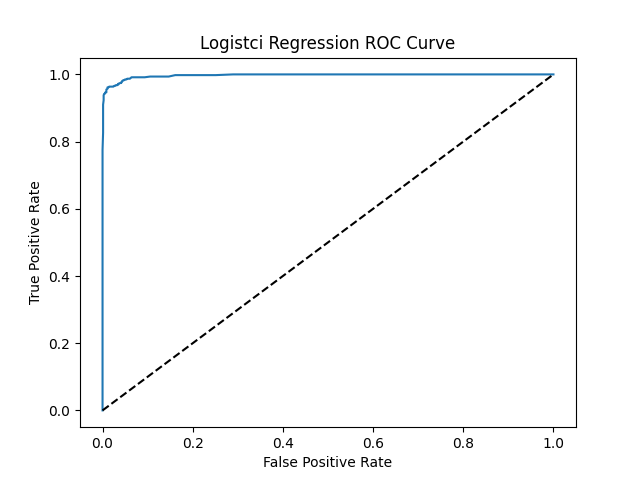
\includegraphics[width=1\linewidth]{LogisticROC.png}
    \caption{ROC Curve for Logistic Regression}
\end{figure}

\subsection{Airi's Progress}

For this project, Airi is implementing two methods: naive bayes and random forest.

Naive Bayes is a group of probabilistic machine learning algorithms based on applying Bayes' theorem with the assumption of independence between features. This assumes that the presence or absence of one feature does not affect the presence or absence of any other feature within a class, and calculates the probabilities of each class label given the values of the features from the input. The class with the highest probability is then selected as the predicted class label for the given input.

Random Forest is an ensemble learning method that combines multiple decision trees to improve the performance and reduce overfitting. Each decision tree is constructed by randomly selecting a set of features and samples from the training set. This randomization helps to make a model less sensitive to noise and outliers in the data, and outperforms other algorithms.